\section{Introduction}
%Background%
Graphs have been widely used to model the complex relationships between objects, such as social networks~\cite{hamilton2017inductive}, academic networks~\cite{getoor2005link}, and biological networks~\cite{gilmer2017neural}. 
In recent years, graph representation learning has shown its effectiveness in capturing the irregular but related complex structures in graph data~\cite{hamilton2017inductive}. 
As an important topology characteristic, hierarchical structures are ubiquitous in many real-world graphs, such as the hypernym structure in natural languages~\cite{NickelK17Poincare,PoincareGlove}, the subordinate structure of entities in the knowledge graph~\cite{balazevic2019multi,wang2020h2kgat}, and the cascade structure of information propagation in social networks~\cite{zubiaga2018detection}. 
In our work, we focus on studying the tree-like structure\footnote{We interchangeably use the terms \textit{heirarchy} and \textit{tree-like structure} in this paper. } which exists extensively in real-world networks~\cite{Krioukov2010Hyperbolic}. 


\begin{figure}[ht]
	\centering
	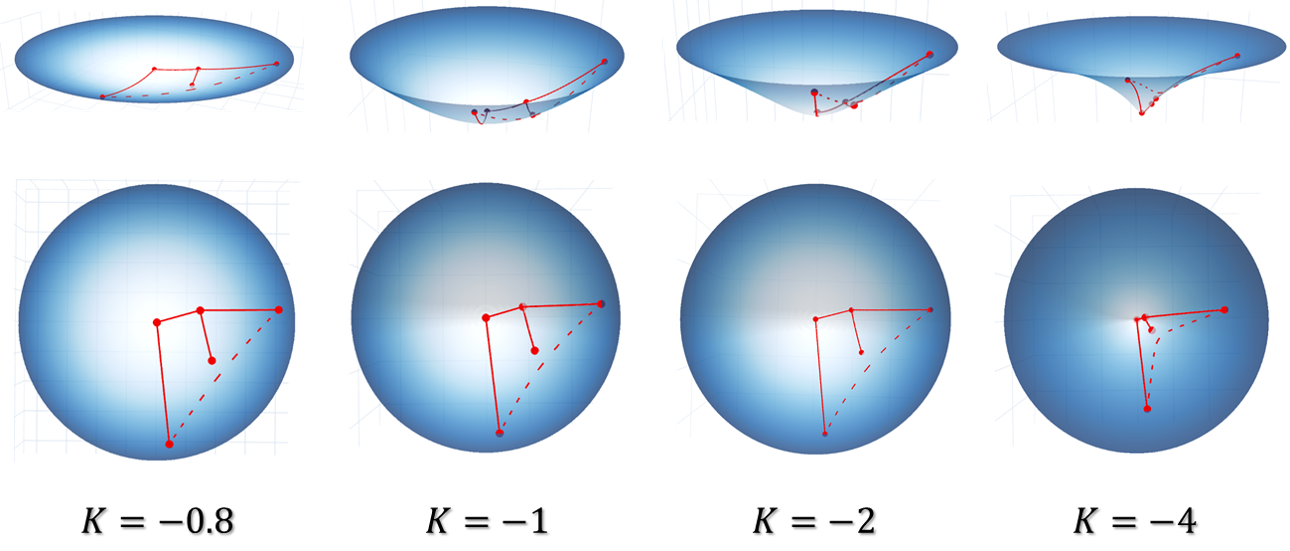
\includegraphics[width=0.45\textwidth]{figure/example_1.png}
	\caption{An example of a hyperbolic distance (\textcolor{red}{dash line}) between two nodes on a binary tree in hyperbolic spaces with different curvatures}
	\label{example_1}
\end{figure}

%Weaknesses of exiting works%
With the advantages of better capturing the hierarchical structures of graphs compared with the Euclidean space, hyperbolic space has been introduced into Graph Neural Networks to achieve better learning performance and interpretability~\cite{NickelK17Poincare}. 
To learn the graph representations in hyperbolic space, Hyperbolic Graph Neural Networks (HGNNs) extend the node feature aggregation of Graph Neural Networks (GNNs) into hyperbolic space. 
HGNNs combine hyperbolic geometric embedding and GNNs, and effectively fuse the node features and the hierarchical structures to acquire the superior node representation for graphs. 

However, a major limitation of existing HGNNs is that they cannot adaptively choose the appropriate hyperbolic space to represent the graphs with different degrees of tree-like structures.
Thus, even though most real-world graphs have tree-like structures, they have different degrees of ``how tree-like a graph is''. 
In this paper, we use Gromov’s $\delta$-hyperbolicity~\cite{adcock2013tree} to measure the degree of tree-like structures of a graph. 
Existing HGNNs provide great expressiveness for high hyperbolicity (more like a tree) graph data, but it shows poor performance in node representation of graphs with low hyperbolicity (less like a tree) ~\cite{HGCN_ChamiYRL19}. 


%Problem presentation%
To investigate this problem, we review hyperbolic geometry and related studies~\cite{cannon1997hyperbolic,Krioukov2010Hyperbolic}, and we were inspired by the curvature which can be used to measure any hyperbolic geometry similarity to Euclidean geometry.
We illustrate an intrinsic connection between hyperbolic curvature and hierarchies of graphs in Figure~\ref{example_1}. 
The examples show that different curvatures significantly affect distance metric in hyperbolic space. 
We can observe that the hyperbolic distance between two nodes in different hyperbolic spaces is approximately equal to the length of shortest path in the tree or the Euclidean distance.
In deep learning frameworks, HNN~\cite{HNN:GaneaBH18} presents that with the curvature going to zero, the hyperbolic distance metric is approximate identical to the Euclidean distance metric. 
The distance measures determine the retention of the hierarchy when embedding graphs into hyperbolic spaces with different curvatures. 
Therefore, a natural problem is, “\textit{Can we make a hyperbolic geometric learning model automatically learn the appropriate curvature to obtain desirable adaptability for different graphs with tree-like structure?}” 

%Challenges%
However, there are two major challenges to adaptively find the optimal hyperbolic curvature to improve the learning ability of HGNNs. 
The one is learning curvature and node representation together may lead to training instability since the updating curvature will continuously change the entire hyperbolic embedding space. 
Existing work~\cite{HGCN_ChamiYRL19} takes curvature as a parameter to learn node representations of the graph. However, instead of learning the accurate curvature in training process, it only slightly adjusts the curvature to make the node representation learning converge in a relatively stable hyperbolic space.
The other one is learning curvature with optimization methods is difficult because there is no strict and formal mathematical method to map curvature and hierarchy of the graph, which can change the hierarchy-preserving capability of hyperbolic space through different distance metric. 



%Proposed method%
To address the above challenges, we propose a novel \textbf{A}daptive \textbf{H}yperbolic \textbf{G}raph \textbf{N}eural \textbf{N}etwork via Multi-Agent \textbf{R}einforcement Learning named \textbf{RAHGNN}. 
The basic idea is that we take the downstream task as the environment in reinforcement learning and calculate the feedback reward based on the hyperbolic node representations.
Specifically, we design two agents: the adaptive curvature explore agent (ACE-Agent) and the hyperbolic graph neural network agent (HGNN-Agent). 
The adaptive curvature explore agent (ACE-Agent) is designed to independently learn the optimal curvature in a broad range of the parameter space based on reinforcement learning. 
The hyperbolic graph neural network agent (HGNN-Agent) with variable curvature is designed to learn the node representations in hyperbolic space with a particular curvature. 
To fully ensure learning both curvature exploration and graph representations in hyperbolic space, we propose a multi-agent reinforcement learning framework to learn curvature and node representations collaboratively. 
The optimized goal is the two cooperative agents have a Nash equilibrium. 
In this way, the curvature can adaptively adjust to the distance metric of embedded space for different graphs with complex hierarchical topologies.
Extensive experiments on typical real-world datasets demonstrate a significant and consistent improvement in model quality with competitive performance. 
We have also visualized the graph in hyperbolic space to provide an intuitive understanding of how different curvatures affect the model's capability of capturing the hierarchy. 
We summarize our contributions as follows: 
\vspace{-0.4em}
\begin{itemize}[leftmargin=*]
\item We make a observation and analysis of the adaptability problem of GNNs to graphs with different hierarchical topologies in hyperbolic space, and we transform the adaptability problem into an optimal curvature exploration problem in hyperbolic space. 
\item We propose a novel hyperbolic graph representation learning framework with superior adaptive capability based on multi-agent reinforcement learning. 
To our best knowledge, it is the first attempt to utilize reinforcement learning in hyperbolic machine learning. 
\item To solve the two key problems of learning curvature and HGNN at the same time, we design the ACE-Agent and HGNN-Agent to learn the curvature and HGNN respectively, and cooperatively train their rewards to reach Nash equilibrium based on multi-agent reinforcement learning. 

\end{itemize}
